%======================================================================
\chapter{Photocatalysis of \texorpdfstring{CO\textsubscript{2}}{CO2}}\label{chap.co2}
\markright{Photocatalysis of \texorpdfstring{CO\textsubscript{2}}{CO2}}
%======================================================================

%======================================================================
\section{Introduction}
%======================================================================

Only 6 years after \ce{Re^I} complexes using 2,2'-bipyridine were characterized, Hawecker, Lehn, and Ziessel showed the effectiveness of the compound for the photocatalytic reduction of \ce{CO2}\autocite{hawecker1983}. Since then, many have shown the efficacy of a wide range of $\alpha$-diimino complexes for the reaction\autocite{hawecker1986, kurz2006, portenkirchner2014} and expansion of the systems to bimetallic complexes with ruthenium and osmium as electron transfer agents has produced a wide range of results\autocite{rossenaar1996, takeda2008, tamaki2013}. The mechanism of reduction has been subject of some debate: while mechanisms have been proposed since Lehn et. al. soon after their original publication\autocite{hawecker1986}, modifications have been submitted routinely over the past decades\autocite{hayashi2003, morris2009, takeda2008, grills2010, agarwal2011, agarwal2012a, agarwal2012b, keith2013}. The development of a novel terdentate geometry and the associated increase in photon absorption at lower energies of the catalyst warranted investigation of the \ce{CO2} reduction capabilities, having overcome the criticism of only utilizing high energy photons \autocite{kutal1985}. 

%======================================================================
\section{Photocatalytic Reactions with New Compounds}
%======================================================================

The photocatalytic cycle is, simply, a photon-induced \gls{ac.mlct}, followed by the extraction of an electron from a sacrificial reductant. This radical, negatively charged species sheds the anion, opening up a reaction site. Reaction between a \ce{CO2}, a proton (from the decomposition of the reductant or elsewhere), and the catalyst yields any number of \ce{CO}, \ce{H2O}, formate (\ce{HCO2-}), or carbonate (\ce{CO3H-}), depending on the mechanistic pathway. Further discussion and a proposal of a new mechanism geometry based on computational and experimental data can be read in \autoref{chap.mech}.

%----------------------------------------------------------------------
\subsection{Conditions}
%----------------------------------------------------------------------

Reaction conditions in use in literature have remained typically unchanged since the original papers. A mixture of \gls{ac.dmf} with either \gls{ac.teoa} or \gls{ac.tea} at a 5:1 ratio is used to make a 1.0 mM solution of catalyst, with `excess' (depending on reference, a 1.1 to 25 molar ratio) electrolyte salt (typically \ce{Et4NX} or \textit{t}-\ce{Bu4NX}, where X = halide from catalyst) added as a stabilizer. Solutions are degassed by bubbling of \ce{CO2} and a consistent headspace is left to form over the solution. The reaction is monitored via \gls{ac.gc} analysis of the headspace, using a HP gas chromatograph with a 15 m CARBONPLOT column with 0.320 mm inner diameter and 1.50 $\mu$m film in a 40~$^\circ$C oven. The instrument is fitted with a \gls{ac.tcd}, and, while using He as a carrier gas, is able to resolve \ce{CO} and \ce{CO2} completely.  

%----------------------------------------------------------------------
\subsection{Experimental Results}
%----------------------------------------------------------------------

Both bidentate and terdentate \ce{$\kappa$^n(terpy)Re(CO)_{5-n}X} (n=2, 3) \textbf{2.1} and \textbf{2.2} complexes show no activity for \ce{CO2} reduction. Modification of testing time, light source, product analysis methods, solvent, sacrificial reductant, pH, presence of electrolyte, presence of \ce{H2O}, or variation of anion (X=Cl, Br, OTf, CN) shows no change of this inactivity. Testing of \ce{$\kappa$^2(bipy)Re(CO)3Cl} under the same reaction and testing conditions shows production of approximately 6 mL \ce{CO} from \ce{CO2} (~20\% conversion) in 1 hour of photolysis with visible ($\lambda$ \textgreater 400 nm) light, verifying the method, isolating the catalyst as the ineffective species. 

%======================================================================
\subsection{Rationalization of Results}\label{ss.rationalization}
%======================================================================
\todo{TEOA insertion, maybe clear is a acid, formate, carbonate, tricarbonylcation or other complex?}

Kurz \textit{et al.} demonstrated the requirement for fluorescence for successful catalytic candidates\autocite{kurz2006}. The explanation for this is the requirement for a stable, long-lasting excited state, with lifetime greater than that of the timescale required for electron abstraction from the sacrificial amine. The observed fluorescence demonstrates the lack of non-radiative relaxation pathways, considered to be an analogue for the extended lifetime of the excited state. Sample \textbf{2.2} shows only poor fluorescence. While the complex is able to absorb light across the spectrum, and has \gls{ac.homo} to \gls{ac.lumo} transitions with high enough energy\footnote{Electrochemical reduction of \ce{CO2} in similar environments takes 1.7-2.1 V, equivalent to \gls{ac.homo}-\gls{ac.lumo} transitions from 590-750 nm\autocite{grills2014}.} for the catalyzed reduction of \ce{CO2} to \ce{CO}, it appears as if the catalysis is not initiated due to a short excited state lifetime. Fluorescence data presented in \autoref{chap.newchem}, at \autoref{ss.fluorescence} shows the lack of strong fluorescence in terdentate sample \textbf{2.2}.

Explanation for the lack of \ce{CO} production observed in the attempted photochemical reduction of \ce{CO2} by bidentate sample \textbf{2.1} and others must come from another angle. These samples are quite fluorescent, emission from the powder sample can be seen with the naked eye with simulation by a 405 nm laser pen under ambient light environments. Importantly, two clues come from the reaction mixture: under intense visible light in the presence of \ce{CO2} the compound bleaches to a very faint yellow-green and colour does not return after storage in the dark, bubbling of new \ce{CO2}, or other manipulations. Secondly, a mixture of sacrificial amine, \gls{ac.dmf}, and catalyst \textbf{2.1} in ratios identical to what is required in the reaction mixture changes colour from a yellow to a deep red irreversibly after 5 days at ambient temperature.

\begin{scheme}[!htb]
 \begin{center}
  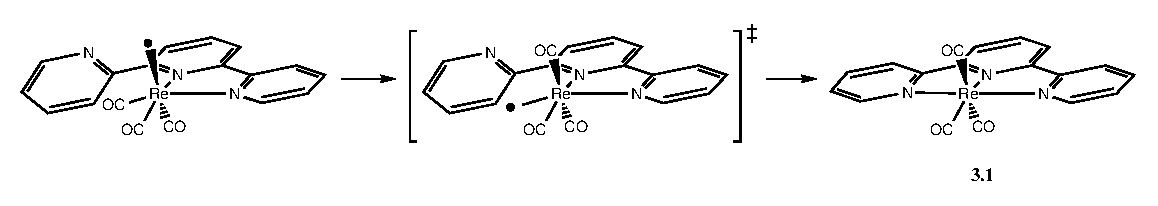
\includegraphics[clip=true, width=120mm, keepaspectratio]{images/tricarbscheme.eps}
 \end{center}
\caption[Reorganization from catalytic eximer to form \textbf{3.1}]{Formation of \textbf{3.1} from catalytic excimer via reorganization of carbonyls and chelation of the pendant arm.}
\label{scheme.tricarbonyl}
\end{scheme}

These variations provide some opportunity for identifying methods of deactivation. The bleaching (formation of a very pale yellow-green to clear species) may be due to the loss of the halide, followed by carbonyl reorganization and pendant arm complexation to form \textbf{3.1}, see \autoref{scheme.tricarbonyl}. This scheme is available to the mechanism via well known processes, lability of carbonyl groups around a metalc entre is well established. The resulting compound, \ce{[$\kappa$^3-(terpy)-Re(CO)3]+}, appears to not have been isolated in literature previously, direct comparisons to experimental colour or UV-Vis is not possible. However, \gls{ac.tddft} calculations with the same parameters used in \autoref{chap.newchem} (B3LYP functional, with a mixed LanL2DZ and TZVP basis set) demonstrate an absorption spectra with very little visible contributions, blueshifted from the catalyst \textbf{2.1}, as shown in \autoref{fig.uvvistricarb}. This corresponds to the bleaching and colour changes seen in the reaction mixture. 

\begin{figure}[!htbp]
 \begin{center}
  \includegraphics[clip=true, keepaspectratio, width=120mm]{images/tricarbcatuvvisstruct.eps}
 \end{center}
\caption[Structure and absorption spectra of proposed \ce{[$\kappa$^3-(terpy)-Re(CO)3]+}]{Computational structure (inset) and predicted UV-Vis absorption spectra of \ce{[$\kappa$^3-(terpy)-Re(CO)3]+}}
\label{fig.uvvistricarb}
\end{figure}

The appearance of the irreversible red product may be the formation of triethanolamine-catalyst adducts\autocite{morimoto2013}. In the presence of DMF, TEOA has been shown to bind to the open site of the excimer via the amine's oxygen atom. This is susceptible to insertion of \ce{CO2} to form a --\ce{OC(O)C}--\ce{CH2CH2N(CH2CH2OH)2} group. \Gls{ac.dft} studies on these two compounds suggest that they may be a coloured species, with predicted UV-Vis showing lower energy absorption than the catalyst itself (a red shift), demonstrated in \autoref{fig.ishitani}.

\begin{figure}[!htbp]
 \begin{center}
  
\includegraphics[clip=true, keepaspectratio, width=120mm]{images/ishitani.eps}
 \end{center}
\caption[]{}
\label{fig.ishitani}
\end{figure}

\todo{ishitani figure}






